\documentclass[11pt,aspectratio=43,ignorenonframetext,t]{beamer}
% Uses fontspec - assumes compiled with LuaLaTeX or similar
% The above \documentclass is for making slides. If making handouts use:
%\documentclass[11pt,a4paper]{article} 
%\usepackage{beamerarticle}
%\setjobnamebeamerversion{main.beamer}

% See https://github.com/CASSON-LAB/uom_beamer_template
% for details on license, further useage information and similar
%%%%%%%%%%%%%%%%%% DOCUMENT SETUP %%%%%%%%%%%%%%%%%%

% Presentation settings
\mode<presentation>{
  \usetheme[framenumber,titleframestart=1]{UoM_alex}
  \usefonttheme{professionalfonts} % using non standard fonts for beamer
  \usefonttheme{serif}             % set font to Arial
  \usepackage{fontspec}
  \setmainfont[Ligatures=TeX]{Arial}
}

% Handout settings
\mode<article>{
  \usepackage{fullpage}                  % use full page
  \usepackage{fontspec}                  % set font to Arial
    \setmainfont[Ligatures=TeX]{Arial}
  \setlength{\parskip}{1.5\baselineskip} % correct beamer line spacings
  \setlength{\parindent}{0cm}
  \usepackage{enumitem}
    \setlist[itemize]{topsep=0pt}
  \definecolor{uomlinkblue}{HTML}{0071BC}
}


% Packages

% Configurando layout para mostrar codigos C++
\usepackage{listings}
\lstset{
  language=Java,
  basicstyle=\ttfamily\small, 
  keywordstyle=\color{blue}, 
  stringstyle=\color{red}, 
  commentstyle=\color{red}, 
  extendedchars=true, 
  showspaces=false, 
  showstringspaces=false, 
  numbers=left,
  numberstyle=\tiny,
  breaklines=true, 
  backgroundcolor=\color{green!10},
  breakautoindent=true, 
  captionpos=b,
  xleftmargin=0pt,
}

\usepackage{graphicx}  % for graphics files
  \graphicspath{ {./fig/aula5} }
\usepackage{amsmath}   % assumes amsmath package installed
  \allowdisplaybreaks[1] % allow eqnarrays to break across pages
\usepackage{amssymb}   % assumes amsmath package installed 
\usepackage{hyperref} % add hyperlinks to document. Settings are for accessiblity
  \hypersetup{
    colorlinks=true,
    linkcolor=uomlinkblue,
    filecolor=uomlinkblue,      
    urlcolor=uomlinkblue,
	pdflang={en-GB},
}
\usepackage[document]{ragged2e} % left aligned text for accessibility
% experimental - does fundamentally work, if with quite a bit of effort
%\usepackage{axessibility} % LaTeX readable equations for accessibility
%  \tagpdfsetup{tabsorder=structure,uncompress,activate-all,interwordspace=true}
%  \pdfextension catalog{/Lang (en-GB)}
%  \RequirePackage{luacode}
%  \directlua{require("axessibility.lua")}
\usepackage{unicode-math} % unicode maths for accessibility
\usepackage{pdfcomment} % for alt text for accessibility
\usepackage{rotating}  % allow portrait figures and tables
\usepackage{subfigure} % allow matrices of figures
\usepackage{float}     % allows H option on floats to force here placement
\usepackage{multirow}  % allows merging of rows in tables
\usepackage{tabularx}  % allows fixed width tables
\usepackage{ctable}    % modifies \hline for use in table
\usepackage{bm}        % allow bold fonts in equations
\usepackage{pgf}       % allow graphics manipulation
\usepackage{media9}    % allow interactive flash files to be embedded
  \addmediapath{../media}
\usepackage{etoolbox}
  \makeatletter \preto{\@verbatim}{\topsep=0pt \partopsep=0pt} \makeatother  
  
% Custom commands
\newcommand{\matlab}{\emph{\sc{Matlab}}}
\newcommand{\maple}{\emph{\sc{Maple}}}
\newcommand{\simulink}{\emph{\sc{Simulink}}}
\newcommand{\dc}{d.c.}
\newcommand{\ac}{a.c.}
\newcommand{\rms}{RMS}
\newcommand{\wgn}{{\tt wgn}}
\newcommand{\sus}[1]{$^{\mbox{\scriptsize #1}}$}
\newcommand{\sub}[1]{$_{\mbox{\scriptsize #1}}$}
\newcommand{\chap}[1]{Chapter~\ref{#1}}
\newcommand{\sect}[1]{Section~\ref{#1}}
\newcommand{\fig}[1]{Fig.~\ref{#1}}
\newcommand{\tab}[1]{Table~\ref{#1}}
\newcommand{\equ}[1]{(\ref{#1})}
\newcommand{\appx}[1]{Appendix~\ref{#1}}
\newcommand{\degree}{\ensuremath{^\circ}}
\newcommand{\Vrms}{Vrms}
\newcommand{\Vpp}{V\sub{pp}}
\newcommand{\otoprule}{\midrule[\heavyrulewidth]}         
\newcolumntype{Z}{>{\centering\arraybackslash}X}  % tabularx centered columns 
\makeatletter \DeclareRobustCommand{\em}{\@nomath\em \if b\expandafter\@car\f@series\@nil \normalfont \else \bfseries \fi} \makeatother
\newcounter{example_number} % keep track of the example questions



%%%%%%%%%%%%%%%%%% FRONT MATTER %%%%%%%%%%%%%%%%%%
\title{Desenvolvimento de Software}
\subtitle{Aula 5}
\author{Prof. Me. Juliana Costa-Silva}
\begin{document}
%%%%%%%%%%%%%%%%%% TITLE SLIDE %%%%%%%%%%%%%%%%%%
\mode<presentation>{ \frame{\titlepage \label{slide:a}}} 
%\begin{figure}[!ht] 
%\fbox{\includeslide[width=\textwidth]{slide:a}} \end{figure}



%%%%%%%%%%%%%%%%%% NEW SLIDE %%%%%%%%%%%%%%%%%%
\clearpage 
\mode<presentation>{\begin{frame}{Na aula de hoje...}
  \setbeamertemplate{section in toc}[sections numbered]
  \tableofcontents[hideallsubsections]
\end{frame}}
%----------------------------------------------------------------------------
%----------------------------------------------------------------------------
\section{static}
\mode<presentation>{\begin{frame}{Static}
  \begin{itemize}
    \item Atributos e métodos estáticos são compartilhados por todos os objetos criados a partir daquela classe.
   \item Existe apenas uma única cópia do método e/ ou atributo que esta associada com a classe e não com alguma instância criada da classe (objetos).
  \end{itemize}
  \begin{columns}
    \begin{column}{0.4\textwidth}
      \begin{block}{Atributos e métodos estáticos}
      pertencem à classe
     \end{block}

    \end{column}
    \begin{column}{0.4\textwidth}
     \begin{block}{Atributos e métodos não-estáticos}
      pertecem ao objeto
     \end{block}
    \end{column}
  \end{columns}

\end{frame}}
%----------------------------------------------------------------------------
\mode<presentation>{\begin{frame}{static}
  Restrições:
    \begin{itemize}
      \item um método estático, \textbf{\textcolor{blue}{NÃO}} pode acessar variáveis de instância;
      \pause \item um método estático, \textbf{\textcolor{blue}{NÃO}} pode se referenciar a métodos de instância.
    \end{itemize}
\end{frame}}
%----------------------------------------------------------------------------
\mode<presentation>{\begin{frame}{static}

  \small{ 
\lstinputlisting[linerange={3-8}]{cod/Estatico.java}
  }
\end{frame}}
%----------------------------------------------------------------------------
\mode<presentation>{\begin{frame}{static}

   \small{ 
\lstinputlisting[linerange={3-15}]{cod/TestaEstatico.java}
  }
\end{frame}}
%--------------------------------------------e--------------------------------
%----------------------------------------------------------------------
\section{Atividade}
\mode<presentation>{\begin{frame}{Atividade}
  \begin{enumerate}
   \item Modele um funcionário. Ele deve ter o nome do funcionário, o departamento onde trabalha, seu salário (double), a data de entrada no banco (String), seu RG (String) e um valor booleano que indique se o funcionário está na empresa no momento ou se já foi embora. Você deve criar alguns métodos de  acordo com sua necessidade. 
    \item Além deles, crie um método bonifica que aumenta o salário do funcionário de acordo com o parâmetro passado como argumento. Crie, também, um método demite , que não recebe parâmetro algum, só modifica o valor booleano indicando que o funcionário não trabalha mais aqui.
  \end{enumerate}
\end{frame}}
%--------------------------------------------------------
\mode<presentation>{\begin{frame}{Atividade}
  \begin{enumerate}
   \item Transforme o modelo em uma classe Java. Teste-a, usando uma outra classe que tenha o main. Você deve criar a classe do funcionário chamada Funcionario, e a classe de teste você pode nomear como quiser. A de teste deve possuir o método main. Um esboço das classes:
  \end{enumerate}
  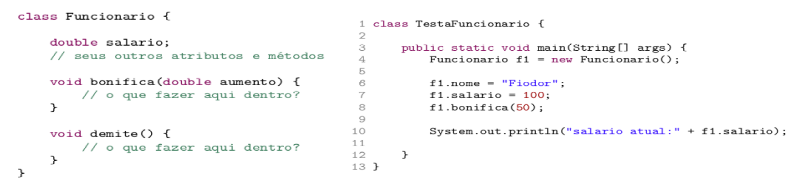
\includegraphics[height=0.3\paperheight]{classes_AEP1.png} \\
\end{frame}}
%-------------------------------------------------------------
\mode<presentation>{\section{Atividade}
\begin{frame}{Atividade de Aula}
  \begin{enumerate}
   \item Implemente o método depositar, na classe conta.
   \item Lembre-se que ele deve atualizar o saldo do cliente;
   \item Teste o método criado.
   \item Envie o código desenvolvido em aula, como atividade de aula.
  \end{enumerate}
\end{frame}}
%------------------------------
\section{Leitura recomendada}
\mode<presentation>{\begin{frame}{Leitura complementar}
 Para mais informações sobre JAVA, leia:\\
	\begin{columns}
	\begin{column}{0.5\textwidth}
	 Capítulo 3 a 7:\\
	 \cite{deitel2017java}
	\end{column}
	\begin{column}{0.4\textwidth}
	
\includegraphics[height=0.6\paperheight]{fig/aula1/deitel2017java.png} 
	\end{column}
	\end{columns}
\textcolor{red}{DISPONÍVEL NA BIBLIOTECA FÍSICA E VIRTUAL}
\end{frame}}

 %----------------------------------------------------------------------------
 
 \mode<presentation>{\begin{frame}{Referências}%[allowframebreaks]
 \small
 \begin{center}
 	\bibliographystyle{apalike}
	 \bibliography{ref_aula_progI}
 \end{center}
 \end{frame}}

\begin{figure}[!ht] \fbox{\includeslide[width=\textwidth]{slide:z}} \end{figure}
Text for notes goes here. 
\begin{itemize}
  \item List 1. 
  \item List 2. 
\end{itemize}


%%%%%%%%%%%%%%%%%% END MATTER %%%%%%%%%%%%%%%%%%
\end{document}